\chap{Zustand: Mach nicht immer dasselbe (Fortgeschritter Modus)}\label{ch.states}

Ein Programm in VPL ist eine Liste von Ereignis-Aktions-Paaren. \emph{Alle} Ereignisse werde eins nach dem anderen überprüft, ob sie stattfinden und falls ja, wird die dazugehörige Aktion ausgelöst. Danach beginnt die Überprüfung von vorne. Wir möchten nun, dass einige Ereignis-Aktions-Paare zu einem bestimmten Zeitpunkt aktiv sind und andere nicht. 

Zum Beispiel in Kapitel ~\ref{ch.line}, falls der Roboter vom Isolierband abkommt, möchten wir, dass er nach links oder nach rechts dreht, um das Isolierband zu suchen, je nach dem, von welcher Seite her er das Isolierband ''verloren'' hat. Wir werden zwei Ereignis-Aktions-Paare benötigen: eines, um den Roboter nach links zu drehen, wenn er das Isolierband rechts verlassen hat und ein zweites um nach rechts zu drehen, wenn er das Isolierband links verlassen hat. 

%Zustände werden in VPL im \emph{fortgeschrittenen} Modus verwendet. Klicken Sie auf \blksm{advanced}, bevor Sie mit den folgenden Projekten arbeiten.

\sect{Klopf, klopf}

In vielen Programmen haben wir einen Schalter benutzt, um ein Verhalten des Roboters auszulösen und einen anderen Schalter, um dieses Verhalten wieder zu stoppen. Wenn wir aber an den Startschalter eines Computers denken, haben wir denselben Schalter, um den Computer ein- oder auszuschalten. Der Schalter \emph{weiss} in welchem Zustand er sich gerade befindet: \bu{eingeschaltet} oder \bu{ausgeschaltet}.

Schreiben Sie ein Programm, das die Lichter des Roboters einschaltet, falls er berührt wird und wieder ausschaltet, wenn er ein zweites Mal berührt wird.

{\raggedleft \hfill Beispielprogramm \bu{tap-on-off.aesl}}

Das Verhalten kann auf einfache Art mit einem \textit{Zustandsdiagramm} dargestellt werden:

\begin{center}
\begin{picture}(240,45)
\thicklines
%\put(0,0){\framebox(240,40){}}
\put(20,20){\circle{40}}
\put(0,0){\makebox(40,40){\textsf{aus}}}
\put(220,20){\circle{40}}
\put(200,0){\makebox(40,40){\textsf{ein}}}
\put(40,30){\vector(1,0){160}}
\put(0,30){\makebox(240,10){\textsf{klopfen $\rightarrow$ einschalten}}}
\put(200,10){\vector(-1,0){160}}
\put(0,10){\makebox(240,10){\textsf{klopfen $\rightarrow$ ausschalten}}}
\end{picture}
\end{center}

Im Diagramm sind zwei Zustände durch Kreise angezeigt, die mit den Namen des Zustandes \bu{ein} und \bu{aus} angeschrieben sind. Der Roboter kann von dem Zustand  \bu{ein} zum Zustand \bu{aus} und zurück wechseln, aber nur durch das Befolgen der Instruktionen die auf den Pfeilen angegeben sind. Die Instruktionen beschreien, wann ein Übergang zu einem anderen Zustand geschehen kann und was dann genau geschieht.

\begin{itemize}
	
	\item \emph{Falls} der Zustand \bu{aus} ist \textbf{\textit{und}} ein \emph{Klopfen} stattfindet, $\rightarrow$ schalten die Lichter \emph{ein} \textbf{\textit{und}} der Zustand wechselt auf \bu{ein}.
	
	\item \emph{Falls} der Zustand \bu{ein} ist \textbf{\textit{und}} ein \emph{Klopfen} stattfindet, $\rightarrow$ schalten die Lichter \emph{aus} \textbf{\textit{und}} der Zustand wechselt auf \bu{aus}.
	
\end{itemize} 

Das fett hervorgehobene Wort ``\textbf{\textit{und}}'' vor dem Pfeil~$\rightarrow$ bedeutet, dass  es \emph{zwei Bedingungen} gibt, die wahr sein müssen, damit der Umschaltvorgang ausgeführt wird. (a) Der Roboter muss in einem bestimmten Zustand sein und (b) das Ereignis muss stattfinden. Wenn beide Bedingungen wahr sind, wird das Umschalten durchgeführt, dies führt dazu, dass der Status geändert und die Aktion ausgelöst wird, die nach dem Pfeil~$\rightarrow$ geschrieben steht.

Es ist wichtig zu verstehen, dass die zwei Teile der Bedingung unabhängig sind. In dem oben aufgeführten Diagramm (hier wiederholt):
\begin{center}
	\begin{picture}(240,45)
	\thicklines
	%\put(0,0){\framebox(240,40){}}
	\put(20,20){\circle{40}}
	\put(0,0){\makebox(40,40){\textsf{aus}}}
	\put(220,20){\circle{40}}
	\put(200,0){\makebox(40,40){\textsf{ein}}}
	\put(40,30){\vector(1,0){160}}
	\put(0,30){\makebox(240,10){\textsf{klopfen $\rightarrow$ einschalten}}}
	\put(200,10){\vector(-1,0){160}}
	\put(0,10){\makebox(240,10){\textsf{klopfen $\rightarrow$ ausschalten}}}
	\end{picture}
\end{center}

erscheint das Ereignis \emph{Klopfen} zweimal, aber die Aktion, ausgelöst durch das Stattfinden eines Ereignisses  \emph{hängt von} dem Zustand des Roboters ab, indem sich dieser gerade befindet.

\vspace*{-1ex}

Bei einem Einzelzustand können unterschiedliche Ereignisse zu unterschiedlichen Aktionen und Übergängen führen. Im nachfolgenden Diagramm wird dies erklärt: 

\begin{center}
	\begin{picture}(240,80)
	\thicklines
	%\put(0,0){\framebox(240,80){}}
	\put(30,42){\circle{30}}
	\put(14,28){\makebox(30,30){\textsf{aus}}}
	\put(220,22){\circle{30}}
	\put(205,8){\makebox(30,30){\textsf{ein2}}}
	\put(40,57){\vector(1,0){160}}
	\put(220,60){\circle{30}}
	\put(205,45){\makebox(30,30){\textsf{ein1}}}
	\put(40,27){\vector(1,0){160}}
	\put(0,60){\makebox(240,10){\textsf{linker Knopf $\rightarrow$ leuchte grün}}}
	\put(0,30){\makebox(240,10){\textsf{rechter Knopf$\rightarrow$ leuchte rot}}}
	\end{picture}
\end{center}

Das Drücken des linken Knopfs während dem Zustand \textbf{aus} führt dazu, dass ein grünes Licht eingeschaltet wird und der Zustand wechselt in den Zustand \textbf{ein1}, während das Drücken des rechten Knopfes \emph{im selben Zustand} dazu führt, dass eine andere Aktion ausgelöst wird, nämlich dass ein rotes Licht eingeschaltet wird und der Zustand in einen anderen Zustand wechselt, nämlich Zustand \textbf{ein2}.

\vspace*{-1ex}

\sect{Die Implementierung der Zustandsdiagramme mit Ereignis-Aktions-Paaren}

\Cref{fig.turn-on-off} zeigt die Implementierung des Verhaltens in der obigen Zustandsmaschine als Ereignis-Aktions-Paar. Der linke Kreis im Block 
\blksm{event-tap-advanced} ist ausgewählt (und erscheint in rot) um anzugeben, dass es sich um ein Erschütterungs-Ereignis handelt (klopfen). 

\importantbox[Der Block Erschütterung/Beschleunigung im fortgeschrittenen Modus]{Der Block für diese Ereignisse unterscheidet sich vom Standard-Modus, da er auch für die Ereignisse der Beschleunigung verwendet wird, die in \cref{ch.angles} beschrieben werden.}

\begin{figure}
	\subfigure[Klopfen, um ein - und auszuschalten]{
		\label{fig.turn-on-off1}
		\includegraphics[width=.4\textwidth]{tap-on-off1}
	}
	\hfill
	\subfigure[Klopfen, um den Zustand zu wechseln]{
		\label{fig.turn-on-off2}
		\includegraphics[width=.4\textwidth]{tap-on-off2}
	}
	\caption{Klopfen führt zu verschieden Resultaten, abhängig vom Zustand}
	\label{fig.turn-on-off}
\end{figure}

Im ersten Ereignis-Aktions-Paar (\cref{fig.turn-on-off1}), besteht das Ereignis aus einem Erschütterungsblock und einer Zustandsanzeige \blksm{state-filter}. Eine Zustandsanzeige stellt vier Teile eines Kreises dar, welche entweder ein- oder ausgeschaltet sein können. Eingeschaltet wird durch orange Farbe angezeigt, ausgeschaltet durch weisse. Im vorliegenden Programm verwenden wir das Viertel oben links um anzugeben, ob die oberen Lichter des Roboters ein- oder ausgeschaltet sind. 

Im Bild \cref{fig.turn-on-off1} ist dieses Viertel weiss was bedeutet, dass das Licht ausgeschaltet ist. Zusammen mit dem Erschütterungs-Ereignis-Block bedeutet dies also, dass \textbf{wenn} der Roboter angeklopft wird \textbf{und} die oberen Lichter ausgeschaltet sind, \textbf{dann} schalte das Licht ein.

Im zweiten Ereignis-Aktions-Paar (\cref{fig.turn-on-off2}) ist das Viertel orange eingefärbt, was bedeutet, dass das Licht eingeschaltet ist. Zusammen mit dem Erschütterungs-Ereignis-Block bedeutet dies, dass \textbf{wenn} der Roboter angeklopft wird \textbf{und} das Licht eingeschaltet ist, \textbf{dann} schalte das Licht aus.

Wenn Sie nochmals das Zustandsdiagramm betrachten, sehen Sie, dass erst die Hälfte der Arbeit erledigt ist. Wenn wir das Licht ein- und ausschalten müssen wir ebenfalls den Zustand ändern: von \bu{aus} auf \bu{ein} oder von \bu{ein} auf \bu{aus}. Um dies zu tun müssen wir bei jedem Paar einen \emph{Zustands}-Aktionsblock hinzufügen (rechts):  
\blksm{action-states}. Mit diesem Block kann man den Zustand für alle vier Viertel auf weiss oder orange ändern. 

Zusammenfassend bedeutet das Programm in \cref{fig.turn-on-off} also folgendes: 

\begin{quote}
	\emph{Wenn} der Roboter angeklopft wird \emph{und} der Zustand \bu{aus} ist,\\
	wechsle den Zustand auf \bu{ein} \emph{und} schalte das obere Licht \bu{ein}.
	
	\emph{Wenn} der Roboter angeklopft wird \emph{und} der Zustand \bu{ein} ist,\\
	wechsle den Zustand auf \bu{aus} \emph{und} schalte das obere Licht \bu{aus}.
\end{quote}

Jedes Ereignis führt also sowohl zu einer Aktion, als auch zu einer Änderung des Zustandes des Roboters. Die Aktion hängt dabei vom \emph{aktuellen} Zustand des Roboters ab.

\sect{Wie viele Zustände stehen zur Verfügung?}

Der Zustandsblock (sowohl als Ereignis als auch als Aktion), kann folgende Farben / Bedeutungen haben:
\begin{itemize}
	\item \textbf{Weiss}: das Viertel ist \emph{ausgeschaltet};
	\item \textbf{Orange}: das Viertel ist \emph{eingeschaltet};
	\item \textbf{Grau}: das Viertel wird nicht berücksichtigt.
\end{itemize}

Ein Beispiel: \blksm{states}; das obere linke und das untere rechte Viertel sind eingeschaltet, das obere rechte Viertel ist ausgeschaltet und das untere linke Viertel wird nicht berücksichtigt. Bringt man den Zustandsblock \blksmpure{states} mit einem Ereignis in Verbindung, bedeutet das, dass das Ereignis eintrifft wenn entweder 
\begin{center}
	\centering
	\makebox{\raisebox{-1.7em}{\includegraphics[height=4em]{states1}}}\quad oder \quad%
	\makebox{\raisebox{-1.7em}{\includegraphics[height=4em]{states2}}}
\end{center}
gegeben sind.

Da jedes der vier Viertel ein- oder ausgeschaltet sein können, gibt es 16 Zustände: 2
$\times$ 2 $\times$ 2 $\times$ 2 = 16 
\begin{quote}
	\bu{(aus, aus, aus, aus), (aus, aus, aus, ein), (aus, aus, ein, aus),\\
		\mbox{}\hspace{3em}\ldots\\
		(ein, ein, aus, ein), (ein, ein, ein, aus), (ein, ein, ein, ein)}.
\end{quote}
\Cref{fig.all-states} zeigt alle 16 möglichen Zustände grafisch auf.

\importantbox{Der aktuellen Zustand des Roboters wird auch im vorderen, oberen Bereich des Roboters angezeigt. Dazu leuchten die diagonal angeordneten Segmente des Lichtkreises entsprechend auf. 	\cref{fig.state-leds} zeigt als Beispiel den Zustand \bu{(ein, ein, ein, aus)}.}

\trickbox[zur Information]{Wenn ein Programm gestartet wird, sind alle Zustände ausgeschaltet. Der initiale Zustand ist also \bu{(aus, aus, aus, aus)}:\quad \blkmed{state-all-off}.}

\trickbox{Falls Sie nicht alle 16 möglichen Zustände verwenden, sondern nur 2 oder 4, dann ist es Ihnen freigestellt, welche Sie verwenden wollen. Wenn Sie andererseits 2 verschiedene Sachen untersuchen wollen, die beide nur 2 verschiedene Werte annehmen können, können Sie für die beiden Sachen zwei unterschiedliche Viertel verwenden. Hier erkennt man, wie nützlich die Möglichkeit ist, Zustände \emph{nicht zu berücksichtigen}.}

\begin{figure}
	\subfigure[Alle möglichen Zustände von Thymio]{
		\label{fig.all-states}
		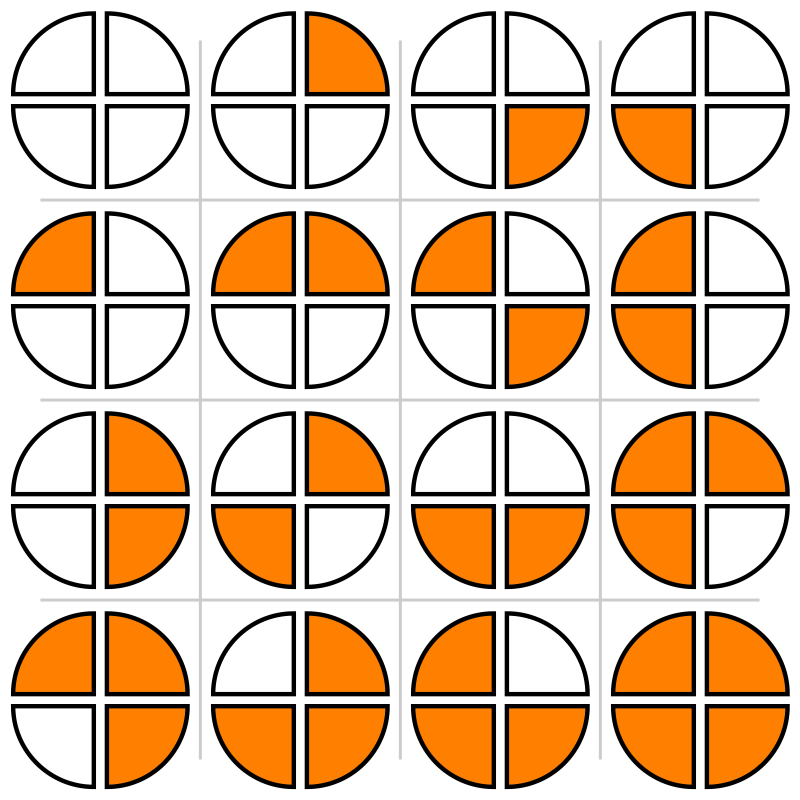
\includegraphics[width=.4\textwidth]{all-states}
	}
	\hfill
	\subfigure[Der Lichterkreis zeigt den Zustand auf]{
		\label{fig.state-leds}
		\includegraphics[width=.4\textwidth]{state-leds}
	}
	\caption{Thymios Zustände und ihre Darstellung}
\end{figure}

\sect{Fang die Maus}

Schreiben Sie nun ein Programm welches das Verhalten einer Katze implementiert, die nach einer Maus sucht: 
Wenn der mittlere Knopf gedrückt wird, dreht sich der Roboter im Gegenuhrzeigersinn (von rechts nach links), um nach der Maus zu suchen. Sobald der Roboter eine Maus mit dem am weitesten rechts sitzenden Sensor entdeckt, dreht er sich im Uhrzeigersinn (von links nach rechts) so lange, bis der mittlere Sensor die Maus entdeckt; dann hält der Roboter an (siehe  (\cref{fig.cat-mouse})).

{\raggedleft \hfill Beispielprogramm \bu{mouse.aesl}}

Das folgende Zustandsdiagramm beschreibt das Verhalten des Roboters: 

\begin{center}
	\unitlength=1.2pt
	\begin{picture}(320,35)
	%\put(0,0){\framebox(320,35){}}
	\put(40,10){\oval(80,20)}
	\put(160,10){\oval(80,20)}
	\put(280,10){\oval(80,20)}
	\put(0,0){\makebox(80,20){\bu{links suchen}}}
	\put(120,0){\makebox(80,20){\bu{rechts suchen}}}
	\put(240,0){\makebox(80,20){\bu{gefunden}}}
	\put( 80,10){\vector(1,0){40}}
	\put(200,10){\vector(1,0){40}}
	\put(40,35){\vector(0,-1){15}}
	\end{picture}
\end{center}

\begin{enumerate}
	\item Wenn der mittlere Knopf gedrückt wird, kommt der Roboter in den Zustand 	\bu{links suchen} und bewegt sich von rechts nach links.
	\item Wenn der Roboter im Zustand \bu{links suchen} ist und mit dem ganz rechts liegenden Sensor eine Maus entdeckt, wechselt er den Zustand in \bu{rechts suchen} und dreht sich von links nach rechts.
	\item Wenn der Roboter im Zustand \bu{rechts suchen} ist und mit dem mittleren Sensor die Maus entdeckt, ändert er in den Zustand \bu{gefunden} und hält an.
\end{enumerate}

Wichtig zu erwähnen ist hierbei, dass wenn die Maus durch den mittleren Sensor entdeckt wird, der Roboter \emph{nur} anhält, \emph{falls} der Roboter sich im Zustand \bu{rechts suchen} befindet. Sonst hält er nicht an (wenn die Maus durch den mittleren Sensor entdeckt wird, sich aber im Zustand \bu{links suchen} befindet). 

%\begin{figure}
%\subfigure[The cat has found the mouse]{\label{fig.cat-mouse}
%\includegraphics[width=0.4\textwidth]{cat-mouse}}
%%	\hfill
%\subfigure[Searching with the rightmost sensor]{\label{fig.mouse2}
%\includegraphics[width=0.6\textwidth]{mouse2}}
%\caption{The robot cat is looking for the mouse}
%\end{figure}

\begin{figure}
	\begin{center}
		\includegraphics[width=0.4\textwidth]{cat-mouse}
		\caption{Die Roboter-Katze sucht nach der Maus}\label{fig.cat-mouse}
	\end{center}
\end{figure}

Wir wollen das beschriebene Verhalten nun Implementieren. Wir stellen den Zustand des Roboters im Viertel oben links dar. Wir wählen weiss für den Zustand \bu{links suchen} und orange für den Zustand \bu{rechts suchen}.
Da das Programm beendet wird, wenn man im Zustand \bu{rechts suchen} die Maus entdeckt, müssen wir den Zustand \bu{gefunden} nicht explizit implementieren.
Bei der Initialisierung sind alle 4 Viertel \bu{aus} (weiss).

Das folgende Ereignis-Aktions-Paar implementiert das Verhalten in Schritt 1: 
\blkc{mouse1}
Wenn der mittlere Knopf gedrückt wird, wird der Zustand geändert auf \bu{links suchen}
\emph{und} der Robotre dreht sich nach links.

Das Ereignis-Aktions-Paar, das den zweiten Schritt implementiert, sieht so aus:
\blkc{mouse2}
Wenn die Maus durch den ganz rechts liegenden Sensor entdeckt wird, während man sich im Zustand \bu{links suchen} befindet, dann ändert der Zustand auf \bu{rechts suchen} \emph{und} der Roboter dreht nach rechts.

Das kleine Quadrat neben dem Sensor ganz rechts wird auf schwarz gestellt, damit das Ereignis nur dann eintritt, wenn die Maus ausschliesslich durch den ganz rechts liegenden Sensor entdeckt wird. 

Schritt 3 wird durch folgendes Ereignis-Aktions-Paar umgesetzt:
\blkc{mouse3}
Wenn die Maus durch den mittleren Sensor entdeckt wurde, während der Roboter sich im Zustand \bu{rechts suchen} befindet, dann hält der Roboter an. 


\trickbox{Experimentieren Sie mit der Position der Maus. Ist diese zu nahe am Roboter, werden die Sensoren zu beiden Seiten die Maus ebenfalls erkennen. Das Ereignis findet jedoch nur statt, wenn die äusseren Sensoren die Maus  \emph{nicht} erkennen}
\bigskip
\exercisebox{\thechapter.1}{
	Schreiben Sie ein Programm, das den Roboter tanzen lässt: Der Roboter soll für zwei Sekunden nach links und dann für drei Sekunden nach rechts drehen. Diese Bewegung soll unendlich oft wiederholt werden.}
\bigskip
\exercisebox{\thechapter.2 (schwierig)}{
	Verändern Sie das Programm ''Einer-Linie-Folgen'' aus dem \cref{ch.line} so, dass der Roboter nach links dreht, falls dieser die Linie auf die rechte Seite verlässt und nach rechts dreht, falls dieser die Linie auf die linke Seite verlässt.
}

